% !TEX root = ../../../main.tex
% 来源：中学数学实验教材·第三册（高中数学）
% 章节：三角函数的图象和性质 / 正弦函数的图象和性质
% 原始文件：7.tex，行 129-151
% 类型：tikz
% ---
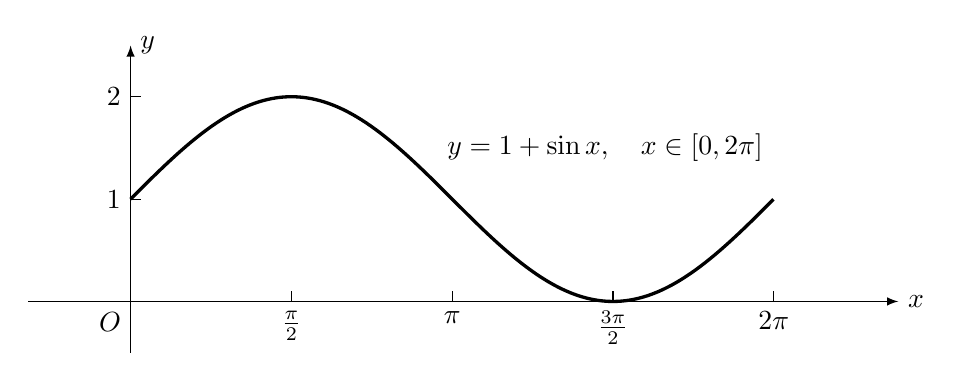
\begin{tikzpicture}[>=latex, scale=1.3]
\draw[->](-1,0)--(7.5,0)node[right]{$x$}; 
\draw [->](0,-.5)--(0,2.5)node[right]{$y$};
    
\draw[domain=0 :2*pi,  samples=1000, very thick] plot(\x, {sin(\x r)+1});
\foreach \x in {1,...,4}
{
    \draw (\x/2*pi,0)--(\x/2*pi,.1);
}
\node at (0,1)[left]{1};
\node at (0,2)[left]{$2$};
\draw (0,1)--(.1,1);
\draw (0,2)--(.1,2);

\node at (-.2,-.2){$O$};
\node at (1/2*pi,0)[below]{$\frac{\pi}{2}$};
\node at (pi,0)[below]{$\pi$};
\node at (3/2*pi,0)[below]{$\frac{3\pi}{2}$};
\node at (2*pi,0)[below]{$2\pi$};

\node at (3,1.5)[right]{$y=1+\sin x,\quad x\in [0,2\pi]$};

\end{tikzpicture}
